\chapter{Binary Tree Reduction}
\label{ch:BinaryTreeSummation}

\newcommand{\numLevels}{\lceil \log_2 N \rceil}
\newcommand{\ffs}{\textrm{ffs}}
\newcommand{\nodesum}{\textrm{sum}\,}

\begin{figure}[H]
\centering
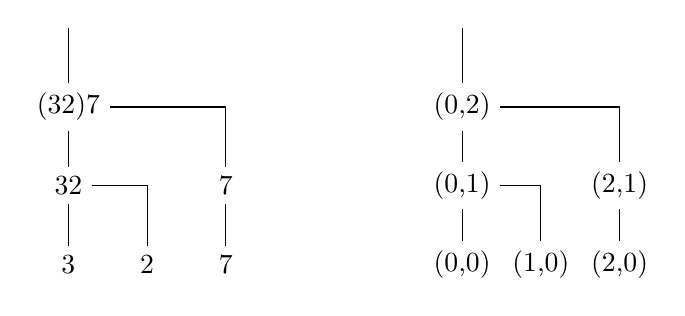
\begin{tikzpicture}
% sample calculation
\node (A) at (0,2) {$(3 \reduce 2) \reduce 7$};
\node (B) at (0,1) {$3 \reduce 2$};
\node (C) at (0,0) {3};
\node (D) at (1,0) {2};
\node (E) at (2,0) {7};
\node (F) at (2,1) {7};
\draw (C) -- (B);
\draw (B) -- (A);
\draw (D) -- (1,1) -- (B);
\draw (E) -- (F);
\draw (F) -- (2,2) -- (A);
\draw (A) -- (0,3);


% coordinate system
\node (A) at (5,2) {(0,2)};
\node (B) at (5,1) {(0,1)};
\node (C) at (5,0) {(0,0)};
\node (D) at (6,0) {(1,0)};
\node (E) at (7,0) {(2,0)};
\node (F) at (7,1) {(2,1)};
\draw (C) -- (B);
\draw (B) -- (A);
\draw (D) -- (6,1) -- (B);
\draw (E) -- (F);
\draw (F) -- (7,2) -- (A);
\draw (A) -- (5,3);
\end{tikzpicture}
\caption{Sample reduction of $3$, $2$ and $7$ and corresponding coordinate system}
\label{fig:coordinateExample}
\end{figure}

In this chapter, we present a special case (where $K = 2$) of the reduction tree from section \ref{sec:ReductionTree}.
To reduce $N$ elements, we construct a binary tree with $N$ leaf nodes,
each corresponding to a single element.
By iteratively connecting adjacent nodes, we produce inner nodes that represent the intermediate result obtained by reducing their children.
After $\numLevels$ levels, all elements have been reduced into a single element represented by the root node.
The left side of figure \ref{fig:coordinateExample} demonstrates this reduction scheme. In a first step, number $3$ and $2$ are reduced.
Since $7$ has no adjacent node, it is left as is. In the next layer, the two remaining elements $5$ and $7$ are reduced, producing the final
result $(3 \reduce 2) \reduce 7$ in the root node.

We can uniquely identify nodes by using \textbf{coordinates} $(x, y)$. The leaf nodes are assigned coordinates
$(0,0)$ through $(N-1,0)$ and the coordinates of inner nodes are obtained by adopting the $x$-coordinate of their left child and incrementing
the $y$-coordinate by $1$. Figure \ref{fig:coordinateExample} shows coordinates for all nodes in a binary tree with $N = 3$ leaf nodes.
An element is said to have index $i$ if its corresponding leaf node has the coordinates $(i,0)$.

As can be easily seen in figure \ref{fig:coordinateExample}, the distance in $x$-direction between the child nodes of inner nodes doubles
with every step in direction $y$. The reduction equation for inner nodes therefore is

$$
\begin{numcases}{\reduceFunc (x,y) =}
\textrm{element with index } x, & for $y = 0$ \label{eq:nodeReduceBaseCase} \\
\reduceFunc (x, y - 1), & for $x+2^{y-1} \geq N$ \label{eq:nodeReducePassthrough} \\
\underbrace{\reduceFunc(x, y - 1)}_{\textrm{left child}} \reduce \underbrace{\reduceFunc (x + 2^{y-1}, y - 1)}_{\textrm{right child}}, & otherwise \label{eq:nodeReduceReduction}
\end{numcases}
$$

Equation \eqref{eq:nodeReduceBaseCase} defines the base case where no further reductions are necessary.
If $N$ is not a power of $2$, there might not always be an adjacent node that can be connected.
In this case, the node is left as is, which is reflected in equation \eqref{eq:nodeReducePassthrough}.
Finally, equation \eqref{eq:nodeReduceReduction} defines the actual recursive reduction strategy of child nodes.
The complete reduction is expressed by applying the $\reduceFunc$-function to the root node: $\reduceFunc (0, \lceil \log_2 N \rceil)$.
To take up the example from figure \ref{fig:coordinateExample} again:
\begin{alignat*}{2}
\reduceFunc (0, \lceil \log_2 N \rceil) &= \reduceFunc(0, 2)  &\hspace{2em}&\rlap{\footnotesize Apply \eqref{eq:nodeReduceReduction}}\\
&= \reduceFunc (0,1) \reduce \reduceFunc(2,1) &&\rlap{\footnotesize Apply \eqref{eq:nodeReduceReduction}} \\
&= (\reduceFunc(0,0) \reduce \reduceFunc (0,1)) \reduce \reduceFunc(2,1) &&\rlap{\footnotesize Apply \eqref{eq:nodeReducePassthrough}} \\
&= (\reduceFunc(0,0) \reduce \reduceFunc (0,1)) \reduce \reduceFunc(2,0) &&\rlap{\footnotesize Apply \eqref{eq:nodeReduceBaseCase}}\\
&= (3 \reduce 2) \reduce 7 &&
\end{alignat*}

From the current point of view, the binary tree reduction has no obvious advantages compared to sequential left-to-right reduction.
It requires the same amount of reduction operations, it even requires more memory since a single accumulator does not suffice to store all intermediate results.
The benefits only become visible if we incorporate \gls{pe}-boundaries into our model.
Recall that our task is to reduce $N$ elements over $p$ \glspl{pe}.
We can split up our binary tree across multiple \glspl{pe} by distributing the elements.
A node with coordinates $(x, y)$ is assigned to a \gls{pe} if the element with index $x$ is assigned to the \gls{pe}.

Figure \ref{fig:distributed_binary_tree} shows an example where nine elements are distributed across three processing elements.
\begin{figure}[H]
\centering
\begin{tikzpicture}
\definecolor{shade1}{rgb}{87 77 104}
\definecolor{shade2}{rgb}{163 133 96}
\definecolor{shade3}{rgb}{198 161 91}

\newcommand{\heightFactor}{0.7}
\newcommand{\treeN}{8}
\newcommand{\subtreeHeight}[2]{\directlua{tex.write(subtree_height(#1,#2))}}
\newcommand{\parentIdx}[1]{\directlua{tex.write(parent(#1))}}
\foreach \x in {0,...,\treeN} {
	\node (idx\x{}) at (\x{},0) {\x};
	
	\draw (idx\x{})
		-- (\x{},\heightFactor * \subtreeHeight{\x}{\treeN}+\heightFactor)
		-- (\parentIdx{\x},\heightFactor * \subtreeHeight{\x}{\treeN}+\heightFactor);
}

\draw [very thick, dashed, rounded corners, teal] (-0.5,-0.5)  rectangle (2.4,3.5);
\draw [very thick, dashed, rounded corners, olive]  (2.6, -0.5) rectangle (5.4,2.5);
\draw [very thick, dashed, rounded corners, brown] (5.6, -0.5) rectangle (8.4,3.5);

\node at (1,-1) {\acrshort{pe} 0};
\node at (4,-1) {\acrshort{pe} 1};
\node at (7,-1) {\acrshort{pe} 2};

\end{tikzpicture}
\caption{Distributed binary tree with $N=9$ leaf nodes and $p=3$ \glspl{pe}.}
\label{fig:distributed_binary_tree}
\end{figure}
The degree of parallelization now becomes visible. Reductions $(0) \reduce (1)$, $(4) \reduce (5)$ and $(6) \reduce (7)$ can all be performed in parallel, since
they do not depend on any external data and are located on different \glspl{pe}.
Other calculations do however require communication between the \glspl{pe}.
A node is called \gls{pe}-intersecting whenever one of its child node is assigned to a different \gls{pe}.
In our example in figure \ref{fig:distributed_binary_tree}, the parent nodes of the leaf nodes $3$ and $8$ are examples of \gls{pe}-intersecting nodes.

\section{Message counts}
The main hinderance to efficient parallelization as outlined in the previous section is the need for synchronization between \glspl{pe} because of data dependencies in the form of \gls{pe}-intersecting nodes.
The target implementation utilizes the \gls{mpi} to communicate between different \glspl{pe} and since the messages are small (one double precision float point value occupies 8 bytes or 64 bits), the total number of messages is a good indicator of the communication overhead.
Under the assumption that no message buffering or any other form of bundling is employed, the message count is equal to the number of \gls{pe}-intersecting nodes.

\begin{figure}
\centering
\begin{subfigure}{0.7\textwidth}
\centering
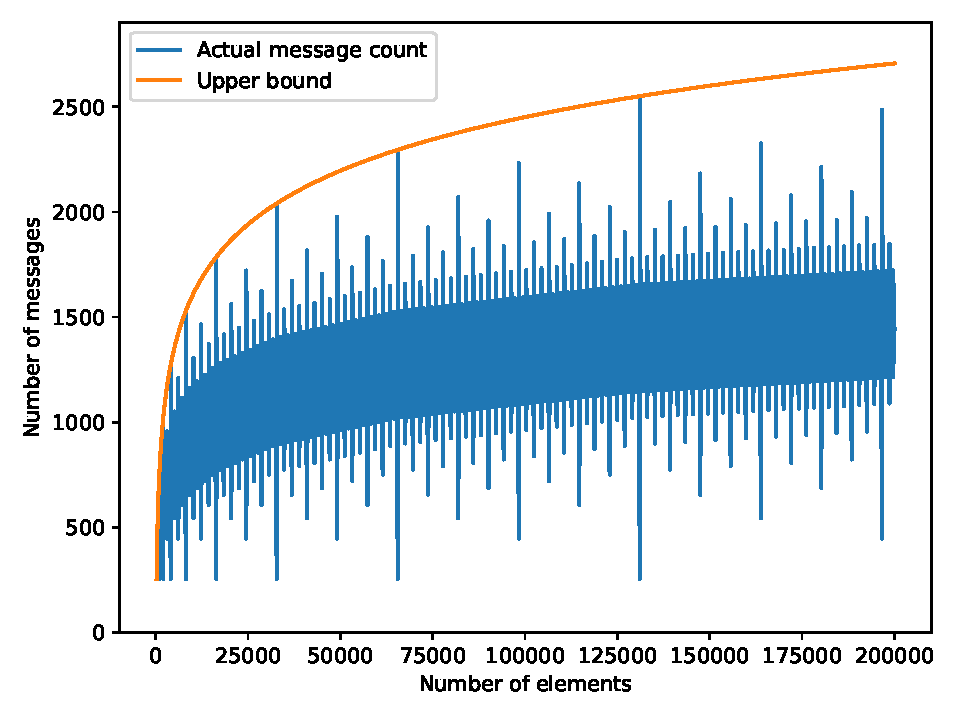
\includegraphics[scale=0.7]{figures/message_count_256.pdf}
\caption{Remaining elements assigned to the lower ranks}
\label{fig:messageCount256}
\end{subfigure}
\hfill
\begin{subfigure}{0.7\textwidth}
\centering
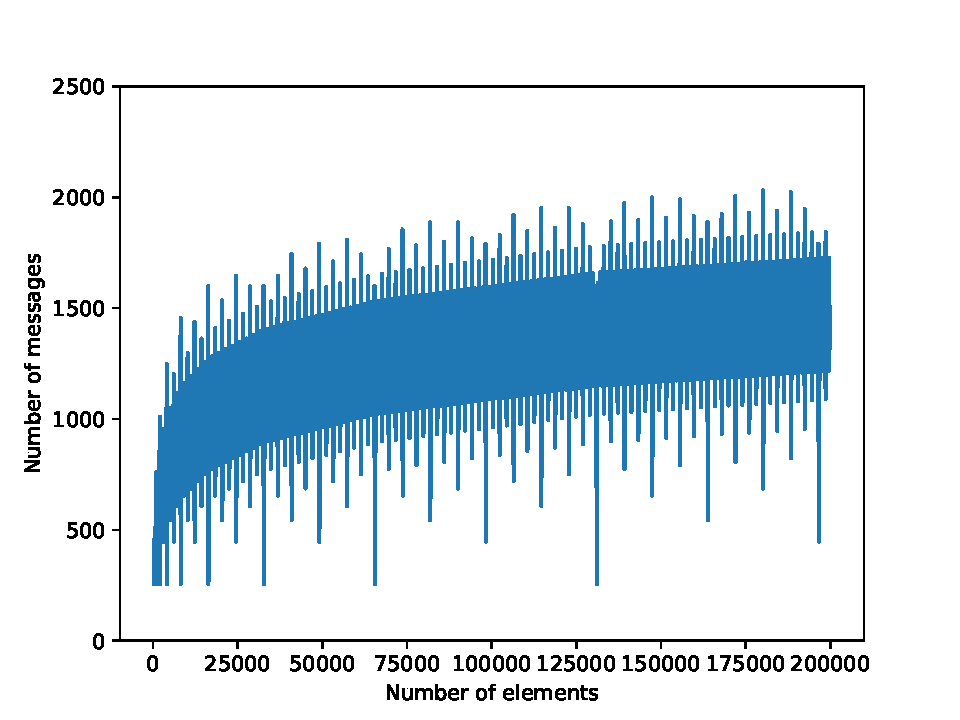
\includegraphics[scale=0.7]{figures/message_count_256_remainder_at_end.pdf}
\caption{Remaining elements assigned to the higher ranks}
\label{fig:messageCount256RemainderAtEnd}
\end{subfigure}

\caption{Simulated message counts for different dataset sizes on a cluster with $p=256$ \glspl{pe}}
\end{figure}

Figure \ref{fig:messageCount256} shows the number of messages depending on the data set size.
The function behaves chaotically and displays large differences in message counts for small differences in dataset sizes.
The lower bound of message counts is $p - 1$, since all \glspl{pe} with a rank larger than $0$ must send at least one subtotal to the root \gls{pe}.
The global minima is attained at $N = 2^i * p$, where $i \in \mathbb{N}$.
Local maxima can be observed at $N = 2^i * p + 1$, directly following the global minima.
This most likely is an effect of the remainder distribution if $N \bmod p \neq 0$, since some of the message count spikes can be eliminated if the remaining elements are placed on the highest instead of the lowest ranks (see figure \ref{fig:messageCount256RemainderAtEnd}).

Equation \eqref{eq:worstcaseMessageCount} is a closed-form approximation of the worst case message count for the unoptimized data distribution where the remaining elements are placed on lower ranks:
\begin{equation}
\label{eq:worstcaseMessageCount}
M_{\textrm{worstcase}}(N) = (p - 1) (\log_2 \Big( \frac{N - 1}{p} \Big) + 1)
\end{equation}
Under the assumption that the number of \glspl{pe} is constant, the message count $M$ therefore is in $O(\log(N))$.